\documentclass[11pt]{article}

\usepackage{amsmath}
\usepackage{amssymb}
\usepackage{array}
\usepackage{caption}
\usepackage{graphicx}

\usepackage[autostyle, english=american]{csquotes}
\MakeOuterQuote{"}
\captionsetup[table]{skip=1pt}

\newcolumntype{M}[1]{>{\centering\arraybackslash}m{#1}}

% margins
\topmargin=-0.45in
\evensidemargin=0in
\oddsidemargin=0in
\textwidth=6.5in
\textheight=9.0in
\headsep=0.25in

\title{605.744: Information Retrieval \\ Problem Set (Module 9)}
\author{Sabbir Ahmed}
\date{\today}

\begin{document}
\maketitle

\begin{enumerate}

    \item (30\%) Give a short definition or explanation of the following concepts:
          \begin{itemize}
              \item web spam

                    \textbf{Answer:} Content on the web that is designed to be artifically favorable in retrieval even though they may be completely irrelevant to the query.

              \item Broders' taxonomy

                    \textbf{Answer:} Classification of search queries by users into 3 categories: informational, navigational, and transactional.

              \item out-degree

                    \textbf{Answer:} In a directed graph, out-degree is the number of edges going out of a vertex.

              \item robots exclusion protocol

                    \textbf{Answer:} Also known as robots.txt, it's used by web pages to inform crawlers on which portions to avoid indexing.

              \item priority queue (in the context of web crawling)

                    \textbf{Answer:} Web crawlers extract URLs from every page they scrape and store them in queues after normalizing them. The URLs can be stored in the queue depending on several factors, including how many links point to each page and their PageRank scores.

          \end{itemize}

    \item (20\%) Describe in your own words the process described in the course text to efficiently identify near duplicate documents in a large collection.

          \textbf{Answer:} Finding near duplicate documents is a lot more difficult than completely duplicate documents, which can be found efficiently by comparing the hashes of the entire documents. One method of identifying near-duplication is by using shingling. This process hashes n-grams of the documents into an integer between 0 and $2^{64}$. These hash sets are intersected and their minimum values are compared to determine the probability of the documents being near-duplicates.

    \item For this problem work with the directed web graph shown below. In the graph there are six nodes: Y, B, F, G, T, R (for the websites Yahoo, Bing, Facebook, Google, Twitter, and Reddit). Use a teleport probability of 0.20. Assume no other pages or links exist beside those shown in the figure.

          \begin{figure}[!ht]
              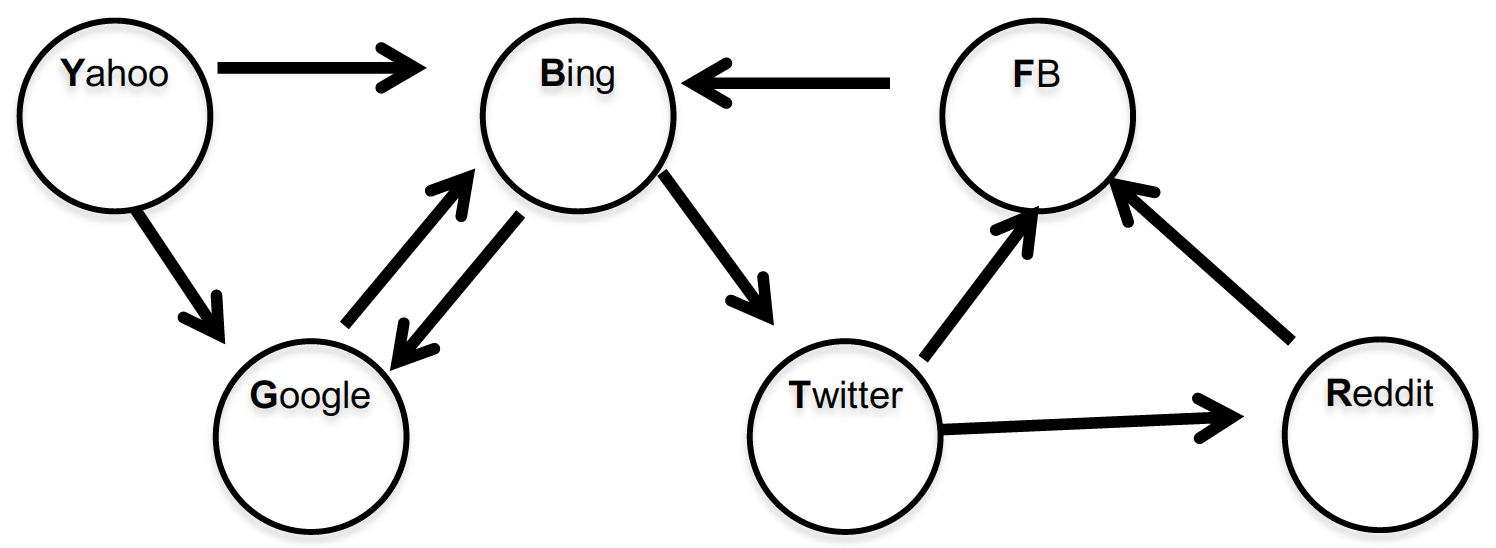
\includegraphics[scale=0.5]{graph.png}
              \centering
          \end{figure}
          \newpage

          \begin{enumerate}
              \item (15\%) Provide (i.e., write) the six recurrence equations that indicate how to iteratively calculate the PageRank score of each page at time t given scores from time t-1.

                    \textbf{Answer:}
                    Using the recurrence equation:
                    \begin{equation}
                        PR(a)=\frac{q}{N}+(1-q)\sum_{i=1}^{n}\frac{PR(p_i)}{C(p_i)}
                    \end{equation}
                    With the values of the sites being initialized to equal probabilities:
                    \begin{table}[!ht]
                        \centering
                        \begin{tabular}[t]{|c|c|c|c|c|c|c|}
                            \hline
                            \textbf{Time} & \textbf{Y} & \textbf{B} & \textbf{F} & \textbf{G} & \textbf{T} & \textbf{R} \\
                            \hline
                            t = 0         & 0.167      & 0.167      & 0.167      & 0.167      & 0.167      & 0.167
                            \\ \hline
                        \end{tabular}
                    \end{table}
                    \begin{align*}
                        PR(Y,t_{i}) & = \frac{0.20}{6}+(0.80) (0)                                                                                          \\
                        PR(B,t_{i}) & = \frac{0.20}{6}+(0.80)\left(\frac{PR(Y,t_{i-1})}{C(Y)}+\frac{PR(F,t_{i-1})}{C(F)}+\frac{PR(G,t_{i-1})}{C(G)}\right) \\
                        PR(F,t_{i}) & = \frac{0.20}{6}+(0.80)\left(\frac{PR(R,t_{i-1})}{C(R)}+\frac{PR(T,t_{i-1})}{C(T)}\right)                            \\
                        PR(G,t_{i}) & = \frac{0.20}{6}+(0.80)\left(\frac{PR(B,t_{i-1})}{C(B)}+\frac{PR(Y,t_{i-1})}{C(Y)}\right)                            \\
                        PR(T,t_{i}) & = \frac{0.20}{6}+(0.80)\left(\frac{PR(B,t_{i-1})}{C(B)}\right)                                                       \\
                        PR(R,t_{i}) & = \frac{0.20}{6}+(0.80)\left(\frac{PR(T,t_{i-1})}{C(T)}\right)
                    \end{align*}

              \item (25\%) Using the brute-force iterative method of calculation shown in the video lecture calculate two iterations of PageRank scores for each page in the graph. Be sure to show scores at times t=0, t=1, and finally at t=2. Report scores using three digits of precision (e.g., 0.247, not 0.2 or 0.24696485932). Show work and do not merely provide a table of values.

                    \textbf{Answer:}
                    \begin{align*}
                        PR(Y,t_{1}) & = \frac{0.20}{6}+0 \\
                                    & = \frac{1}{30}     \\
                                    & = 0.033
                    \end{align*}
                    \begin{align*}
                        PR(B,t_{1}) & = \frac{0.20}{6}+(0.80)\left(\frac{PR(Y,t_{0})}{C(Y)}+\frac{PR(F,t_{0})}{C(F)}+\frac{PR(G,t_{0})}{C(G)}\right) \\
                                    & = \frac{1}{30}+(0.80)\frac{1}{6}\left(\frac{1}{2}+\frac{1}{1}+\frac{1}{1}\right)                               \\
                                    & = \frac{1}{30}+\frac{1}{3}                                                                                     \\
                                    & = 0.367                                                                                                        \\
                        PR(B,t_{2}) & = \frac{1}{30}+(0.80)\left(\frac{0.033}{2}+\frac{0.233}{1}+\frac{0.167}{1}\right)                              \\
                                    & = 0.367
                    \end{align*}
                    \begin{align*}
                        PR(F,t_{1}) & = \frac{0.20}{6}+(0.80)\left(\frac{PR(R,t_{0})}{C(R)}+\frac{PR(T,t_{0})}{C(T)}\right) \\
                                    & = \frac{1}{30}+(0.80)\frac{1}{6}\left(\frac{1}{1}+\frac{1}{2}\right)                  \\
                                    & = \frac{1}{30}+\frac{1}{5}                                                            \\
                                    & = 0.233                                                                               \\
                        PR(F,t_{2}) & = \frac{1}{30}+(0.80)\left(\frac{0.100}{1}+\frac{0.100}{2}\right)                     \\
                                    & = 0.153
                    \end{align*}
                    \begin{align*}
                        PR(G,t_{1}) & = \frac{0.20}{6}+(0.80)\left(\frac{PR(B,t_{0})}{C(B)}+\frac{PR(Y,t_{0})}{C(Y)}\right) \\
                                    & = \frac{1}{30}+(0.80)\frac{1}{6}\left(\frac{1}{2}+\frac{1}{2}\right)                  \\
                                    & = 0.167                                                                               \\
                        PR(G,t_{2}) & = \frac{1}{30}+(0.80)\left(\frac{0.367}{2}+\frac{0.033}{2}\right)                     \\
                                    & = 0.193
                    \end{align*}
                    \begin{align*}
                        PR(T,t_{1}) & = \frac{0.20}{6}+(0.80)\left(\frac{PR(B,t_{0})}{C(B)}\right) \\
                                    & = \frac{1}{30}+(0.80)\frac{1}{6}\left(\frac{1}{2}\right)     \\
                                    & = \frac{1}{30}+\frac{1}{15}                                  \\
                                    & = 0.100                                                      \\
                        PR(T,t_{2}) & = \frac{1}{30}+(0.80)\left(\frac{0.367}{2}\right)            \\
                                    & = 0.180
                    \end{align*}
                    \begin{align*}
                        PR(R,t_{1}) & = \frac{0.20}{6}+(0.80)\left(\frac{PR(T,t_{0})}{C(T)}\right) \\
                                    & = \frac{1}{30}+(0.80)\frac{1}{6}\left(\frac{1}{2}\right)     \\
                                    & = \frac{1}{30}+\frac{1}{15}                                  \\
                                    & = 0.100                                                      \\
                        PR(R,t_{2}) & = \frac{1}{30}+(0.80)\left(\frac{0.100}{2}\right)            \\
                                    & = 0.073
                    \end{align*}
                    \begin{table}[!ht]
                        \centering
                        \begin{tabular}[t]{|c|c|c|c|c|c|c|}
                            \hline
                                  & \textbf{Y} & \textbf{B} & \textbf{F} & \textbf{G} & \textbf{T} & \textbf{R} \\
                            \hline
                            t = 0 & 0.167      & 0.167      & 0.167      & 0.167      & 0.167      & 0.167
                            \\ \hline
                            t = 1 & 0.033      & 0.367      & 0.233      & 0.167      & 0.100      & 0.100
                            \\ \hline
                            t = 2 & 0.033      & 0.367      & 0.153      & 0.193      & 0.180      & 0.073
                            \\ \hline
                        \end{tabular}
                    \end{table}

              \item (5\%) Which page (or pages) has/have the lowest PageRank score after two iterations?

                    \textbf{Answer:} Yahoo has the lowest PageRank score after two iterations with a value of 0.033.

              \item (5\%) Which page (or pages) has/have the highest PageRank score after two iterations?

                    \textbf{Answer:} Bing has the highest PageRank score after two iterations with a value of 0.367.

          \end{enumerate}

\end{enumerate}

\end{document}
